% SVN info for this file
\svnidlong
{$HeadURL$}
{$LastChangedDate$}
{$LastChangedRevision$}
{$LastChangedBy$}

\chapter{Varietà topologiche}
\labelChapter{varietà}

\begin{introduction}
	‘‘BEEP BOOP INSERIRE CITAZIONE QUA BEEP BOOP.''
	\begin{flushright}
		\textsc{NON UN ROBOT,} UN UMANO IN CARNE ED OSSA BEEP BOOP.
	\end{flushright}
\end{introduction}

\section{Varietà topologiche}
%AAA INTRODUZIONE BELLA CERCASI
Si vuole formalizzare il concetto di avere \textit{localmente} la topologia euclidea. 
%BIBLIOGRAFIA
\begin{define}\textsc{Localmente euclideo.}\\
	Uno spazio topologico $X$ si dice \textbf{localmente euclideo}\index{localmente euclideo} di dimensione $n$ se ogni punto di $X$ ammette un intorno aperto omeomorfo ad una palla aperta di $\realset^n$.
\end{define}

\begin{define}\textsc{Varietà topologica.}\\
	Uno spazio topologico $X$ si dice \textbf{varietà topologica}\index{varietà topologica} di dimensione $n$ se $X$ è di \textbf{Hausdorff}, connesso, a base numerabile e localmente euclideo di dimensione $n$.
\end{define}

\begin{examples}
	\begin{itemize}
		\item $\realset^n$ è una varietà topologica di dimensione $n$.
		\item $S^n$ è una varietà topologica compatta di dimensione $n$, infatti grazie alla proiezione stereografica si ha che $S^\setminus\{*\}\cong \realset$.
		\item $\mathbb{P}^n(\realset)$ è una varietà topologica compatta di dimensione $n$.
		\item Ogni aperto connesso di una varietà topologica di dimensione $n$ è una varietà topologica di dimensione $n$.
	\end{itemize}
\vspace{-3mm}
\end{examples}
\begin{observe}
	La dimensione di una varietà topologica è \textit{ben definita} per l'\textit{invarianza della dimensione}.
\end{observe}
\begin{observes}~{}
	\begin{itemize}
		\item Una varietà topologica è \textbf{c.p.a.}.
		\item Se $X$ è una varietà topologica di dimensione $n$ e $Y$ è una varietà topologica di dimensione $m$ allora $X\times Y$ è una varietà topologica di dimensione $n+m$.
	\end{itemize}
%DIMOSTRAZIONE TUTORATO dei due punti precedenti
\end{observes}
\begin{example}
	$T=S^1\times S^1$ è una varietà topologica di dimensione $2$.
\end{example}

\begin{theorema}
	Sia $X$ uno spazio topologico compatto, connesso, \textbf{Hausdorff} e localmente euclideo di dimensione $n$. Allora $X$ è a \textit{base numerabile}, dunque $X$ è una varietà topologica di dimensione $n$.
\end{theorema}
 
\subsection{Dimensione 1}
Analizziamo il caso di varietà topologiche di dimensione $1$, per esempio $\realset$ e $S^1$.
\begin{theorema}
	Ogni varietà topologica di dimensione $1$ è omeomorfo a $\realset$ se \textit{non} è compatta, oppure a $S^1$ se compatta.
\end{theorema}
\begin{example} 
Riconsideriamo l'esempio della \textbf{retta con 2 origini} (sez. \ref{retta 2 origini}, pag. \ref{retta 2 origini}): essa è un quoziente non \textbf{Hausdorff}, dunque \textit{non} è una varietà topologica.
\end{example}
	\subsection{Dimensione 2}
\begin{define}\textsc{Superficie topologica.}\\
	Una varietà topologica di dimensione $2$ si dice \textbf{superficie topologica}\index{superficie!topologica}.
\end{define}
\begin{examples}
	\begin{itemize}
		\item Il \textit{piano} $\realset^2$ oppure $\realset^2\setminus \{n\text{ punti}\}$ sono superfici topologiche di dimensione $2$ \textit{non} compatte.
		\item La \textbf{sfera} $S^2$ è una superficie topologica compatta.
		\item Il \textbf{toro} $T=S^1\times S^1$ è una superficie topologica compatta.
		\item Il \textbf{piano proiettivo} $P=\mathbb{P}^2(\realset)$ una superficie topologica compatta.
	\end{itemize}
\vspace{-3mm}
\end{examples}
Vogliamo dare una classificazione delle superfici topologiche \textit{compatte}. Innanzitutto, esaminiamo alcuni esempi di superfici compatte studiandole sul \textit{modello piano}, di cui daremo successivamente una definizione formale.
\begin{examples} \textsc{Modelli piani.}\\
			\begin{itemize}
		\item Siccome $\mathbb{P}^2(\realset)$ è un quoziente del disco, allora, a meno di omeomorfismo, lo si può anche vedere come un quoziente di $I\times I$ con una relazione di equivalenza sul bordo con \textit{parola} $abab$.
		\begin{center}
		\includegraphics[trim=0cm 0cm 0cm 0cm, clip, scale=0.375]{images/proj.pdf}
		\end{center}
		\item Anche il \textbf{toro} si può vedere come quoziente di $I\times I$ con \textit{parola} $aba^{-1}b^{-1}$.
		\begin{center}
			\includegraphics[trim=0cm 0cm 0cm 0cm, clip, scale=0.375]{images/torus.pdf}
		\end{center}
		\item Vediamo $S^2$ come quoziente di $I\times I$ con \textit{parola} $bb^{-1}a^{-1}a$.
		\begin{center}
			\includegraphics[trim=0cm 0cm 0cm 0cm, clip, scale=0.375]{images/sphere.pdf}
		\end{center}
	\end{itemize}
\vspace{-6mm}
\end{examples}

\begin{observe}
	Sia $P\subset\realset^2$ un \textit{poligono} pieno con un numero \textit{pari} di lati. Sia $\sim$ una relazione di equivalenza che identifica i lati a $2$ a $2$. Allora $S\coloneqq\nicefrac{P}{\sim}$ è una \textit{superficie topologica compatta}, infatti:
		\begin{enumerate}
			\item  $P$ è connesso e compatto $\implies S$ connesso e compatto.
			\item $S$ è localmente euclideo di dimensione $2$. Infatti, sia $p\in S$:
			\begin{itemize}
				\item Se $p$ viene da un punto interno al poligono allora si sceglie un intorno aperto $U$ centrato in tale punto tale che $U\cap\partial{P}=\emptyset$, data la proiezione $\funz \pi P S$, $\pi(U)\cong U$ ed è un intorno aperto di $p$.
				\item Se $p$ viene da un punto interno ad un lato grazie all'identificazione dei lati a due a due si ha che passando al quoziente, cioè un intorno aperto di $p$ omeomorfo ad un disco aperto.
				Se $p$ viene da un vertice, siccome i vertici vengono identificati con i vertici, analogamente al caso dei lati si ottiene un intorno aperto di $p$ in $S$ omeomorfo ad un disco aperto di $\realset^2$.
			\end{itemize}  
			\item $S$ è di \textbf{Hausdorff}.
		\end{enumerate}
	% riguardare la frase, magari separare in un equazione a parte
	Osserviamo che nella relazione di equivalenza due lati vengono identificati nel modo seguente: $l_i\cong\intv$, dunque scelgo un omeomorfismo $l_1\stackrel{\stackrel{\phi}{\sim}}{\longrightarrow} l_2$, $p_1\in l_1 \sim \phi(p)\in l_2$ e $\phi$ manda vertici in vertici.\\
	Il poligono $P$ con la relazione di equivalenza sui lati è detto un \textbf{modello piano}\index{modello piano} della superficie $S$ e può essere schematizzato con una \textit{sequenza di lettere} detta \textbf{parola}\index{parola}. Ad esempio, per la parola $aba^{-1}cbc^{-1}$ si ottiene il modello piano seguente:
		\begin{center}
	\includegraphics[trim=0cm 0cm 0cm 0cm, clip, scale=0.375]{images/modellopiano.pdf}
\end{center}
 Inoltre, il modello piano di una superficie compatta \textit{non è unico}.
\end{observe}

\begin{examples}
	\begin{itemize}
		\item Abbiamo già visto il modello piano di $S^2$ sul \textit{quadrato}; per la costruzione effettuata, possiamo unire la sequenza di lati $ab$ in un unico lato $c$ in modo da ottenere un modello costituito da un poligono \textit{improprio a due lati}, con parola $cc^{-1}$:
		\begin{center}
			\includegraphics[trim=0cm 0cm 0cm 0cm, clip, scale=0.375]{images/sphere2lines.pdf}
		\end{center}
		\item Anche il modello piano di $\mathbb{P}^2(\realset)$ sul \textit{quadrato} può essere trasformato in uno sul poligono a due lati, unificando $ba$ per ottenere un'unico lato $c$ e un modello con parola $cc$:
		\begin{center}
			\includegraphics[trim=0cm 0cm 0cm 0cm, clip, scale=0.375]{images/proj2lines.pdf}
		\end{center}
		\item La \textbf{bottiglia di Klein}\index{bottiglia di Klein} $K$ è la superficie compatta data dal modello piano:
				\begin{center}
			\includegraphics[trim=0cm 0cm 0cm 0cm, clip, scale=0.375]{images/klein.pdf}
		\end{center}
		Confrontiamo la costruzione della bottiglia di Klein con la costruzione del \textit{toro}, vista precedentemente. Innanzitutto otteniamo in entrambi il cilindro $S^1\times I$ con la relazione di equivalenza sul \textit{bordo}; notiamo che nella bottiglia di Klein (il modello inferiore nella figura sotto) il ‘‘verso'' rispetto al quale \textit{incolleremo} i bordi sono uno l'opposto dell'altro.
		\begin{center}
			\includegraphics[trim=0cm 0cm 0cm 0cm, clip, scale=0.375]{images/kleintorus.pdf}
		\end{center}
	Questo comporta che la bottiglia di Klein \textit{non} può essere rappresentata in $\realset^3$; tuttavia, possiamo visualizzarla in modo improprio operando un ‘‘\textit{taglio}'' nella superficie e compenetrando uno dei due estremi del cilindro nella figura, come di seguito.
	 \begin{center}
	 	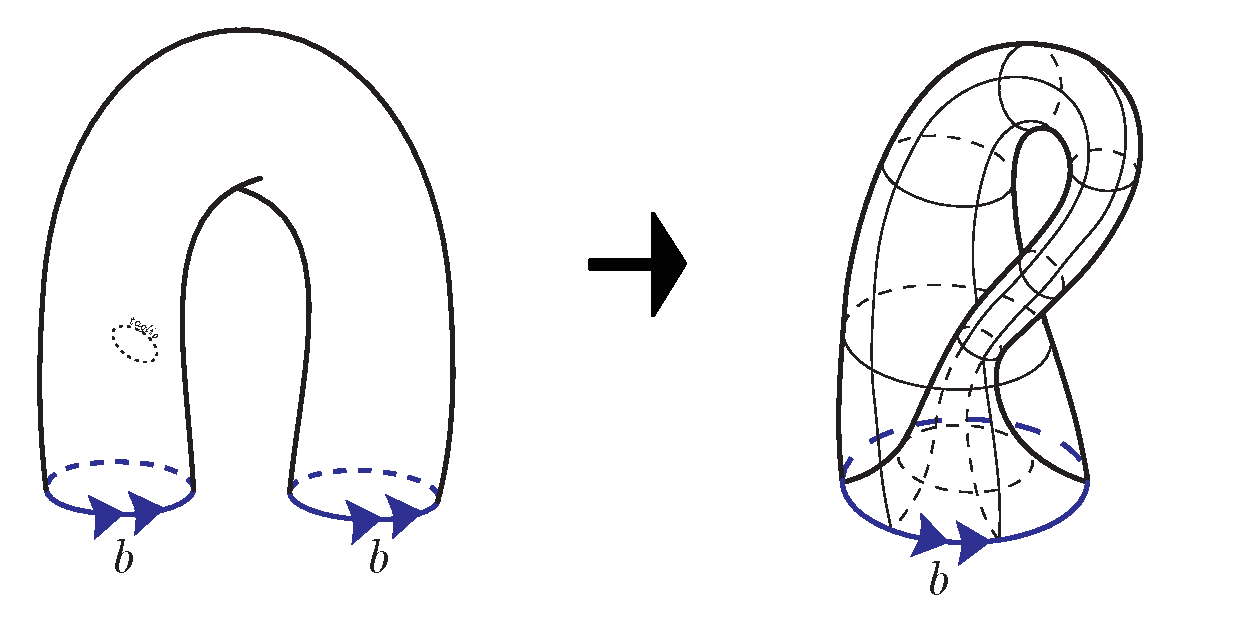
\includegraphics[trim=0cm 0cm 0cm 0cm, clip, scale=0.375]{images/kleinconstruction.pdf}
	 \end{center}
	\end{itemize}
\end{examples}

\section{Somma connessa di superfici compatte}
Siano $S_1$ e $S_2$ superfici compatte e siano $x\in S_1$ e $y\in S_2$. Siano $D_x\subset S_1$ e $D_y\subset S_2$ intorni di $x$ e $y$ rispettivamente, omeomorfi ad un disco chiuso $D\subset\realset^2$:
% https://q.uiver.app/?q=WzAsMixbMCwwLCJEX3giXSxbMSwwLCJEX3kiXSxbMCwxLCJcXHN0YWNrcmVse2h9e1xcc2ltfSJdXQ==
\[\begin{tikzcd}
	{D_x} & {D_y}
	\arrow["{\stackrel{h}{\sim}}", from=1-1, to=1-2]
\end{tikzcd}\]
\begin{center}
	\includegraphics[trim=0cm 0cm 0cm 0cm, clip, scale=0.4]{images/connectedsum1.pdf}
\end{center}
\textit{Togliamo} dalle due superfici gli interni dei dischetti, creando dunque lo spazio:
\begin{equation*}
	Y\coloneqq (S_1\setminus \interior{D_x})\amalg (S_2\setminus \interior{D_y})
\end{equation*}
\begin{center}
	\includegraphics[trim=0cm 0cm 0cm 0cm, clip, scale=0.4]{images/connectedsum2.pdf}
\end{center}
\textit{Incolliamo} ora i due pezzi di $Y$ lungo i bordi dei dischi, cioè mettiamo su $Y$ la seguente relazione di equivalenza:
\begin{equation*}
	x_1\sim y_1 \iff x_1=y_1\text{ oppure } x_1\in\partial{D},\ y_1\in\partial{D}\text{ e } y_1=h(x_1)\text{ (o viceversa)} 
\end{equation*}
\begin{center}
	\includegraphics[trim=0cm 0cm 0cm 0cm, clip, scale=0.4]{images/connectedsum3.pdf}
\end{center}
Vediamo ora qualche fatto che \textit{non} dimostriamo:
	\begin{itemize}
		\item Il quoziente è ancora una superficie topologica, che chiamiamo \textbf{somma connessa}\index{somma!connessa} $S_1\# S_2$  di $S_1$ e $S_2$. 
		\item La somma connessa $S_1\# S_2$, a meno di omeomorfismo, \textit{non dipende} dalle scelte fatte come i punti $x$ e $y$, gli intorni $D_x$ e $D_y$, l'omeomorfismo $h$, ma soltanto da $S_1$ e da $S_2$!
		\item La somma connessa di superfici compatte è, a meno di omeomorfismi, \textit{commutativa} e \textit{associativa}:
		\begin{itemize}
			\item \textsc{Commutativa}: $S_1\# S_2\cong S_2\# S_1$.
			\item \textsc{Associativa}: $\left(S_1\# S_2\right)\# S_3\cong S_1\#\left(S_2\# S_3\right)$.
		\end{itemize}
	\item Se $S_1,\ S_2$ sono superfici compatte, allora anche $S_1\# S_2$ è una superficie topologica compatta.
	\end{itemize}
\begin{observe}
	Sia $X$ una superficie compatta. Allora $X\# S^2\cong X$. Infatti, $S^2\setminus D_y$ è omeomorfismo ad un \textit{disco chiuso} in $\realset^2$. Dato che stiamo togliendo un disco anche ad $X$ per poi aggiungerne un altro, ritroviamo $X$ a meno di omeomorfismi.
	\begin{center}
		\includegraphics[trim=0cm 0cm 0cm 0cm, clip, scale=0.4]{images/connectedsumsphere.pdf}
	\end{center}
\vspace{-6mm}
\end{observe}
\begin{define}\textsc{Somma di tori.}\\
	Indichiamo con $T_g$ la \textbf{somma connessa di }$g\geq 1$ \textbf{tori}:
	\begin{equation}
		T_g=\underbrace{T\# \ldots\# T}_{g\ \text{volte}}\quad g\geq 1\ \left(T_1=T\right)
	\end{equation}
$T_g$ può essere visualizzato sia come ‘‘ciambella con $g$ buchi'' , sia ‘‘come sfera con $g$ manici''.
\begin{center}
	\includegraphics[trim=0cm 0cm 0cm 0cm, clip, scale=0.25]{images/toruschain.pdf}
	\includegraphics[trim=0cm 0cm 0cm 0cm, clip, scale=0.25]{images/spherewithhandle.pdf}
\end{center}
\vspace{-3mm}
\end{define}
\subsubsection{Rappresentazione della somma connessa tramite modelli piani}
\vspace{-3mm}
\begin{minipage}{.74\linewidth}
Supponiamo che $S_1$ e $S_2$ abbiano entrambe un modello piano, rappresentato da una parola.\\
Ad esempio, prendiamo come $S_1$ un \textit{toro}, con parola $a_1b_1a_1^{-1}b_1^{-1}$. Scegliamone un \textit{vertice} e prendiamo un disco $\overline{U}$ passante per il vertice che non tocca il resto del bordo.
\end{minipage}
\begin{minipage}{.25\linewidth}
\begin{center}
	\includegraphics[trim=0cm 0cm 0cm 0cm, clip, scale=0.4]{images/torusmodelconnect1.pdf}
\end{center}
\end{minipage}
Per fare la somma connessa, togliamo $U$:
\vspace{-3mm}
\begin{center}
	\includegraphics[trim=0cm 0cm 0cm 0cm, clip, scale=0.35]{images/torusmodelconnect2.pdf}
\end{center}
\vspace{-3mm}
Facciamo lo stesso con la seconda superficie, $S_2$ (che in questo esempio è anch'essa un toro di parola $a_2b_2a_2^{-1}b_2^{-1}$).
\vspace{-3mm}
\begin{center}
	\includegraphics[trim=0cm 0cm 0cm 0cm, clip, scale=0.35]{images/torusmodelconnect3.pdf}
\end{center}
\vspace{-3mm}
Infine, \textit{incolliamo} lungo i due nuovi lati creati bucando le due superfici:
\vspace{-3mm}
 \begin{center}
 	\includegraphics[trim=0cm 0cm 0cm 0cm, clip, scale=0.35]{images/torusmodelconnect4.pdf}
 \end{center}
Il modello ottenuto è un modello piano per $S_1\# S_2$, la cui parola associata è ottenuta per \textit{concatenazione}:
\begin{equation*}
	\underbrace{a_1b_1a_1^{-1}b_1^{-1}}_{\text{modello piano di }S_1}\underbrace{a_2b_2a_2^{-1}b_2^{-1}}_{\text{modello piano di }S_2}
\end{equation*}
\begin{example}
Il toro $T$ è dato dalla parola $aba^{-1}b^{-1}$. Allora $T_g=T\#\ldots\# T$ ha un modello piano dato dalla parola :
\begin{equation*}
a_1b_1a_1^{-1}b_1^{-1}a_2b_2a_2^{-1}b_2^{-1}\ldots a_gb_ga_g^{-1}b_g^{-1}
\end{equation*}
$T_g$ è un quoziente con $4g$ lati.
\end{example}
\begin{define}\textsc{Somma connessa di $n$ piani proiettivi}
	Preso il \textit{piano proiettivo reale} $P=\proj[2]{\realset}$, definiamo la \textbf{somma connessa di} $n$ \textbf{piani proiettivi} come:
	\begin{equation*}
		P_n=\underbrace{P\# \ldots\# P}_{n\ \text{volte}}\quad n\geq 1\ \left(P_1=P\right)
	\end{equation*}
\vspace{-3mm}
\end{define}
\begin{observe}~\\
	\begin{minipage}{.49\linewidth}
		Studiamo come la \textit{bottiglia di Klein} altro non è che la somma connessa di due piani proiettivi, cioè $K=P\# P=P_2$.\\
		$K$ ha il modello piano quadrato con parola $aba^{-1}b$, mentre invece $P=\proj[2]{\realset}$ ha il modello piano a due lati con parola $cc$.\\
		Pertanto, la somma connessa $P\# P$ ha il modello piano dato dalla parola $ccdd$.
	\end{minipage}
	\begin{minipage}{.49\linewidth}
		\begin{center}
			\includegraphics[trim=0cm 0cm 0cm 0cm, clip, scale=0.3]{images/klein.pdf}
			\includegraphics[trim=0cm 0cm 0cm 0cm, clip, scale=0.3]{images/proj2lines.pdf}
			\includegraphics[trim=0cm 0cm 0cm 0cm, clip, scale=0.3]{images/projdouble.pdf}
		\end{center}
	\end{minipage}
Vogliamo vedere che $aba^{-1}b$ e $ccdd$ danno la stessa superficie. Partiamo dal primo modello e tagliamo lungo la diagonale.
\begin{center}
	\includegraphics[trim=0cm 0cm 0cm 0cm, clip, scale=0.3]{images/kleintoprojdouble1.pdf}
\end{center}
Incolliamo lungo il lato $b$:
\begin{center}
	\includegraphics[trim=0cm 0cm 0cm 0cm, clip, scale=0.3]{images/kleintoprojdouble2.pdf}
\end{center}
Infatti, otteniamo come modello $aaee$, che corrisponde a $P\# P$.
\end{observe}
\begin{lemming}
	\begin{equation}
		T\# P= K\# P=P\# P\# P
	\end{equation}
\vspace{-6mm} %vedremo $T\# K$ (???), non vale la legge di cancellazione per la somma connessa.
\end{lemming}
\begin{demonstration}
	Sappiamo già che, essendo $K=P\# P$, allora $K\# P=P\# P\# P$. Vogliamo invece mostrare ora che $T\# P$ sia uguale a $K\# P$. Facciamo un procedimento di taglia e incolla, partendo da $T\# P$, modello piano con parola $aba^{-1}b^{-1}cc$.
	\begin{center}
			\includegraphics[trim=0cm 0cm 0cm 0cm, clip, scale=0.3]{images/torusplusproj1.pdf}
	\end{center}
Incolliamo lungo $c$:
\begin{center}
	\includegraphics[trim=0cm 0cm 0cm 0cm, clip, scale=0.3]{images/torusplusproj2.pdf}
\end{center}
Otteniamo un modello piano di $T\# P$ che può essere descritto dalla parola $dadbab^{-1}$.\\ Prendiamo adesso $K\# P$, di parola $\underbrace{\delta\beta\delta^{-1}\beta}_{K}\underbrace{\gamma\gamma}_{P}$:
\begin{center}
	\includegraphics[trim=0cm 0cm 0cm 0cm, clip, scale=0.3]{images/kleinplusproj1.pdf}
\end{center}
Incolliamo lungo $\gamma$:
\begin{center}
	\includegraphics[trim=0cm 0cm 0cm 0cm, clip, scale=0.3]{images/kleinplusproj2.pdf}
\end{center}
Otteniamo un modello piano di $K\# P$ che può essere descritto dalla parola $\delta \alpha \delta\beta\alpha\beta^{-1}$, che corrisponde lettera per lettera al modello $T\# P$.
\end{demonstration}
\begin{corollary}
Se $g\geq 1$ e $n\geq 1$ si ha:
\begin{equation}
	T_g\# P_n=P_{n+2g}
\end{equation}
\vspace{-6mm}
\end{corollary}
\begin{demonstration}
	Se $g=1$:
	\begin{equation*}
		T\# P_n=\underbrace{T\# P}_{P_3}\# P_{n-1}=P_3\# P_{n-1}=P\# P_{n+2}
	\end{equation*}
Procediamo per induzione su $g$; se è vero per $g-1$, allora:
\begin{equation*}
	T_g\# P_n=T\# T_{g-1}\# P_n=T\# P_{n+2g-2}=T\# P\# P_{n+2g-3}=P_3\# P_{n+2g-3}=P_{n+2g}
\end{equation*}
\end{demonstration}
\section{Classificazione delle superfici topologiche compatte}
\begin{theorema}\textsc{Classificazione delle superfici topologiche compatte.}\\
Ogni superfici topologica compatta è omeomorfa a $S^2$, $T_g$ per qualche $g\geq 1$ oppure $P_n$ per qualche $n\geq 1$.\\
Inoltre, tali superfici sono tutte distinte, ovvero:
\begin{itemize}
	\item $T_g\ncong T_{g'}$ se $g\neq g'$.
	\item $P_n\ncong P_{n'}$ se $n\neq n'$.
	\item $T_g\ncong P_{n}\ \forall n\geq 1,\ \forall g\geq 1$.
	\item $S^2\ncong T_g\ \forall g\geq 1$.
	\item $S^2\ncong P_n\ \forall n\geq 1$.
\end{itemize}
\vspace{-3mm}
\end{theorema}
\subsection{Triangolazione}
\begin{define}\textsc{Triangolo geometrico.}\\
	Sia $S$ una superficie compatta. Un \textbf{triangolo geometrico}\index{triangolo geometrico} $T$ in $S$ è un applicazione:
	\begin{equation}
		\funz{\phi}{T'}{T\subseteq S}
	\end{equation}
Dove $T'\subseteq \realset^2$ è un triangolo \textit{non} degenere (compreso dell'interno), inteso nel senso tradizionale del termine, mentre $\phi$ è un omeomorfismo.\\
I vertici e i lati di $T$ sono le immagini tramite $\phi$ dei vertici dei lati di $T'$.
\begin{center}
	\includegraphics[trim=0cm 0cm 0cm 0cm, clip, scale=0.3]{images/spheretriangle.pdf}
\end{center}
\vspace{-6mm}
\end{define}
\begin{define}\textsc{Triangolazione.}\\
	Sia $S$ una superficie compatta. Una \textbf{triangolazione}\index{triangolazione} di $S$ è una collezione \textit{finita} di triangoli geometrici $T_1,\ \ldots,\ T_r$ in $S$ tale che:
	\begin{enumerate}
		\item $S=T_1\cup \ldots \cup T_r$.
		\item $\forall i\neq j$ si ha che $T_i\cap T_j$ può essere una di queste tre possibilità:
		\begin{itemize}
			\item $\emptyset$.
			\item Un \textit{vertici} di entrambi i triangoli.
			\item Un \textit{lato} di entrambi i triangoli.
		\end{itemize}
	\end{enumerate}
Una superficie compatta $S$ si dice \textbf{triangolabile}\index{triangolabilità} se ammette una triangolazione.
\end{define}
\begin{example}
	Il \textbf{tetraedro} dà una triangolazione della sfera con $4$ triangoli.
\end{example}
Enunciamo ora un teorema (di cui \textit{non} daremo dimostrazione) che ci servirà successivamente per poter classificare le superfici compatte direttamente con i loro modelli piani associati.
\begin{theorema}\textsc{Teorema di Radò, 1925.}\\
	Ogni superficie compatta è triangolabile.
\end{theorema}
\begin{corollary}
	Ogni superficie compatta $S$ ha un modello piano.
\end{corollary}
\begin{demonstration}
	Per il teorema di Radò, $S$ ammette una triangolazione $T_1,\ \ldots,\ T_r$. Riportiamo gli $r$ triangoli nel piano, con i lati identificati. Incolliamo poi i lati uno ad uno fino ad ottenere un unico poligono con delle identificazioni sui lati.
\end{demonstration}
\subsection{Dimostrazione del teorema di classificazione: prima parte}
La prima parte della dimostrazione del teorema di classificazione si occupa di dimostrare che \textit{tutte le superfici compatte sono omeomorfe a $S^2$, $T_g$ o $P_n$}. Grazie al corollario appena dimostrato, possiamo studiare direttamente il \textit{modello piano} associato alla superficie compatta $S$ in esame, cioè studieremo un \textit{poligono} con i lati identificati a $2$ a $2$.
% note per i disegni
% AGGIUNGERE Note di Topologia Algebrica e Analisi Complessa http://www.science.unitn.it/~perotti/disgeoIII.pdf